\documentclass[12pt,a4paper]{article}
\usepackage[unicode,colorlinks=true]{hyperref}
\usepackage[czech]{babel}
\usepackage[utf8]{inputenc}
\usepackage[T1]{fontenc}
\usepackage{lmodern}
\usepackage{amssymb}
\usepackage{amsmath}
\usepackage{graphicx}
\textwidth 16cm \textheight 24.6cm
\topmargin -1.3cm
\oddsidemargin 0cm

\begin{document}

\setlength{\parindent}{0pt}
\pagestyle{empty}
\noindent

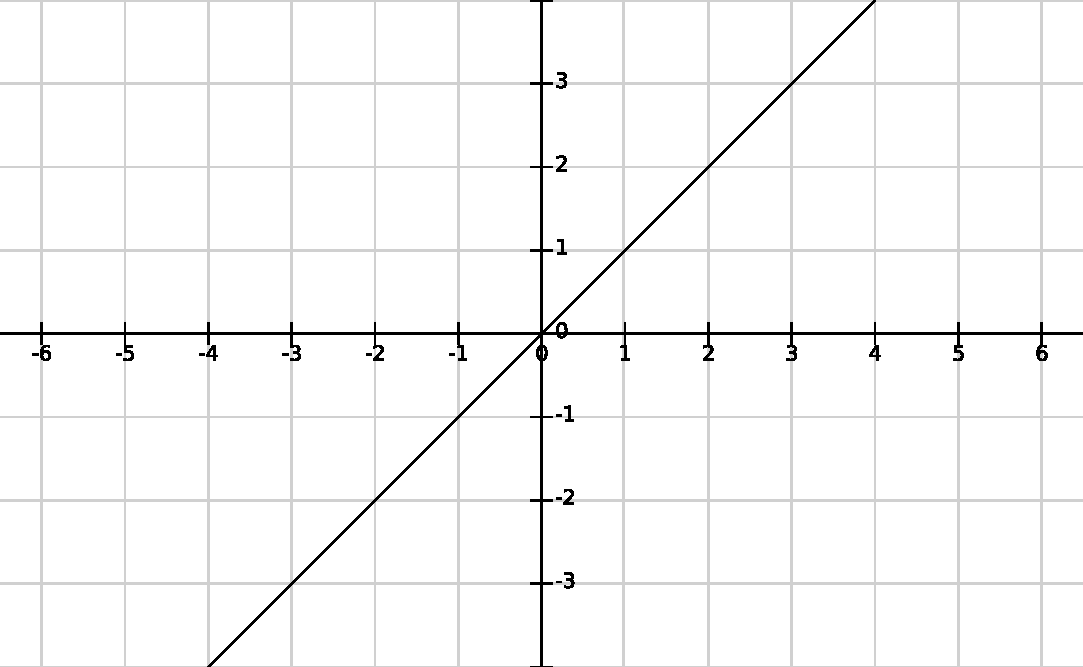
\includegraphics[height=5cm]{x.pdf}
\vspace{1em}
\hspace{1em}
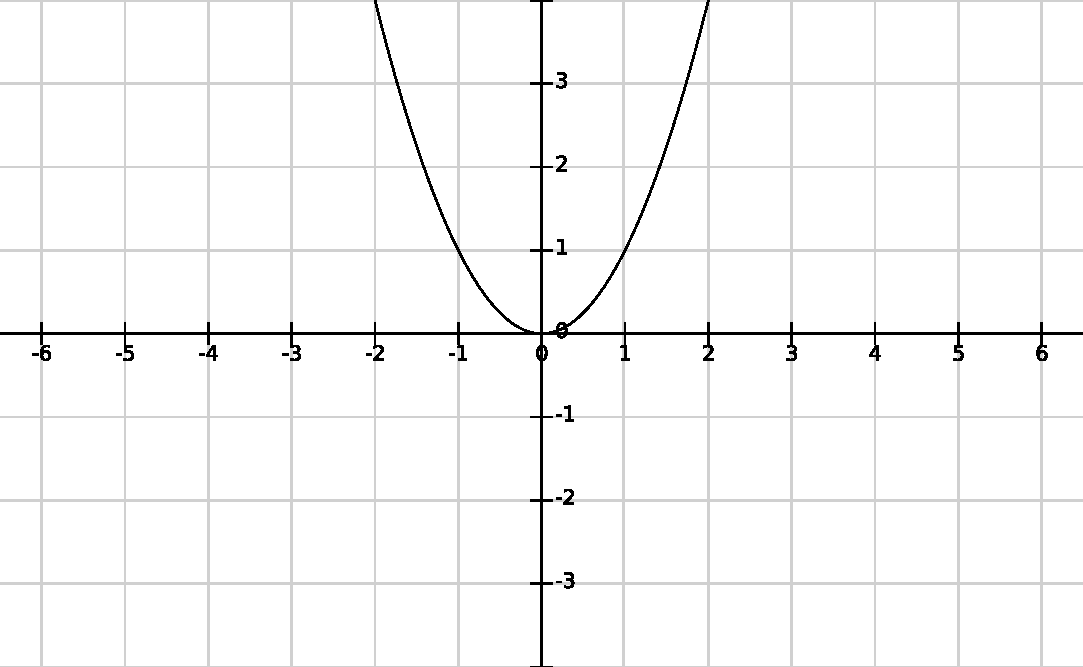
\includegraphics[height=5cm]{x^2.pdf}
\vspace{1em}
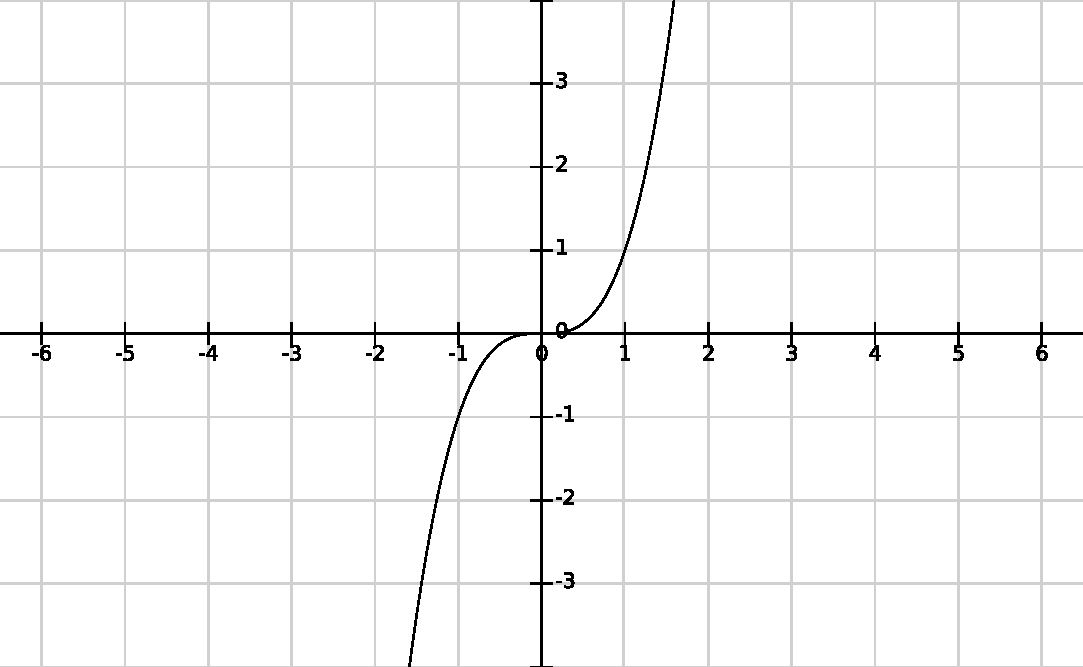
\includegraphics[height=5cm]{x^3.pdf}
\vspace{1em}
\hspace{1em}
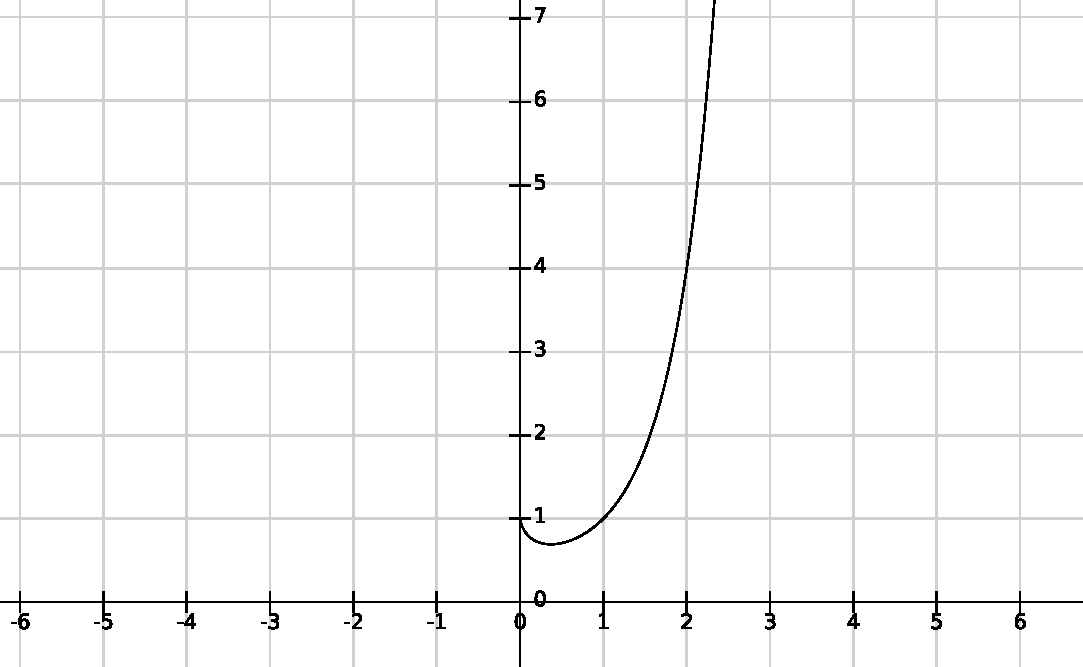
\includegraphics[height=5cm]{x^x.pdf}
\vspace{1em}
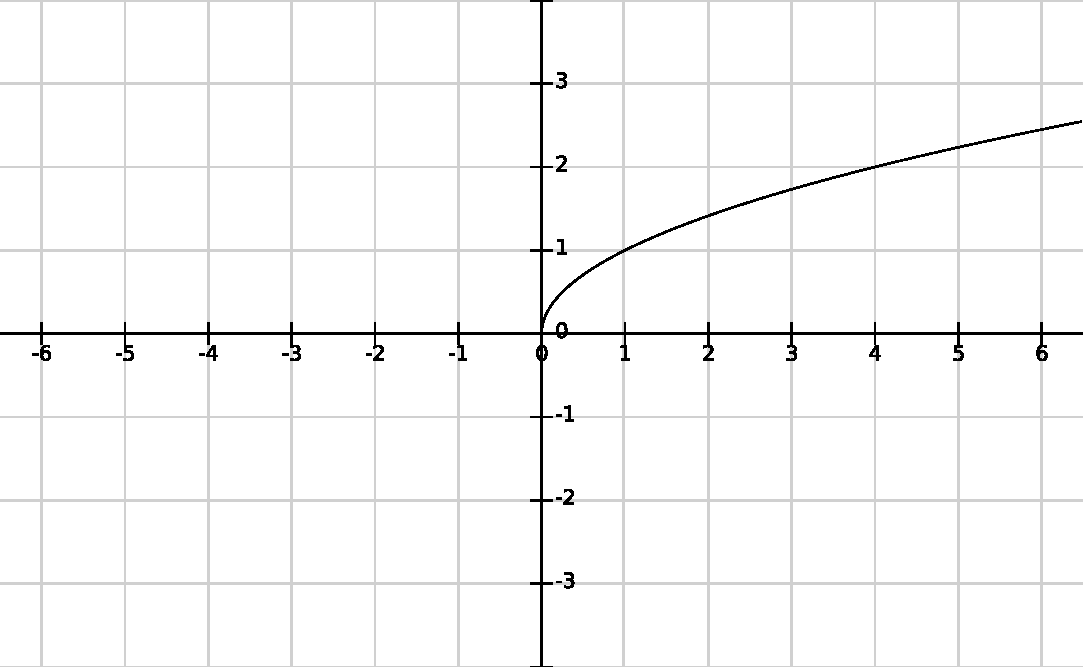
\includegraphics[height=5cm]{sqrtx.pdf}
\vspace{1em}
\hspace{1em}
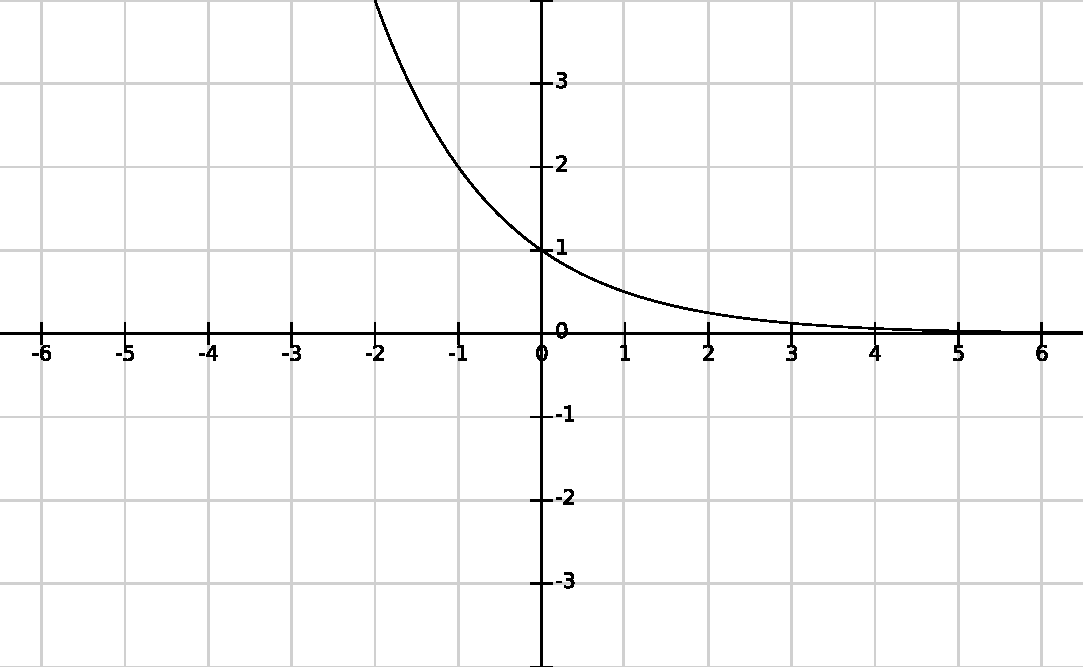
\includegraphics[height=5cm]{2^-x.pdf}
\vspace{1em}
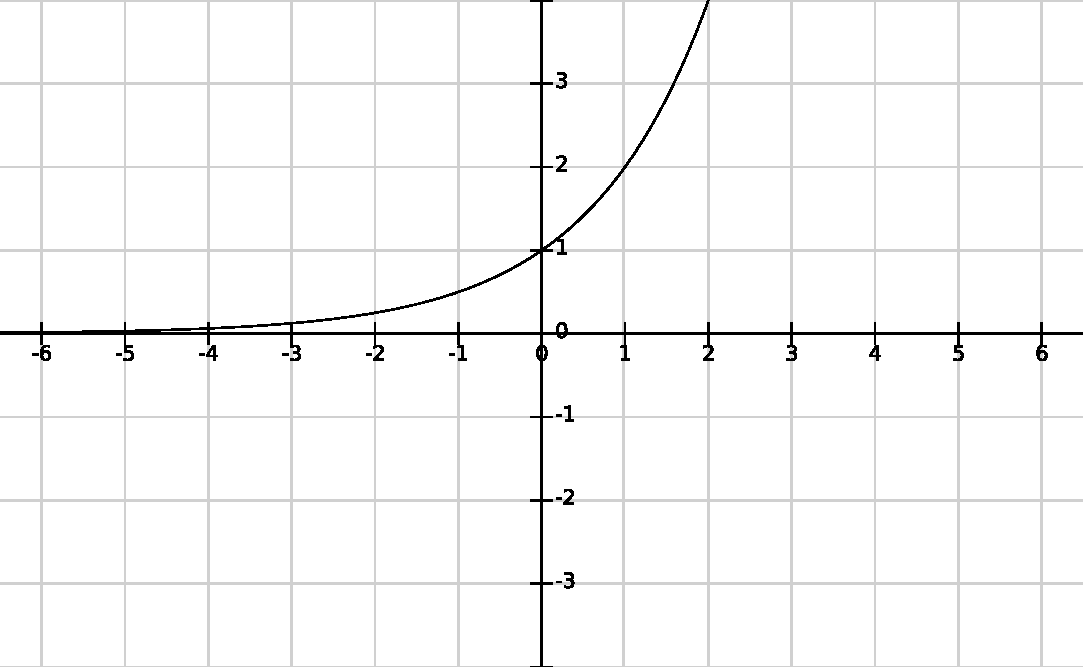
\includegraphics[height=5cm]{2^x.pdf}
\vspace{1em}
\hspace{1em}
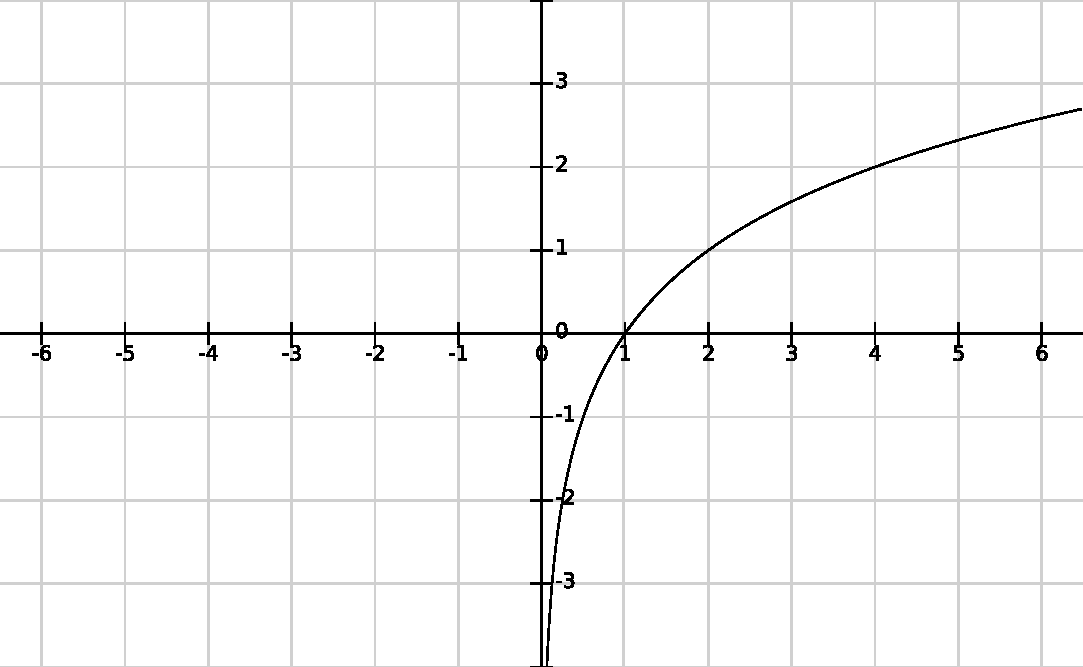
\includegraphics[height=5cm]{log_2x.pdf}

\newpage

\large

\[ x \]
\[ x^2 \]
\[ x^3 \]
\[ x^x \]
\[ \sqrt{x} \]
\[ 2^{-x} \]
\[ 2^x \]
\[ \log_2{x} \]

\begin{align*}
	f(1) &= 1 \\
	f(4) &= 2 \\
	f(8) &= 3 \\
	f(16) &= 4 \\
	&\vdots
\end{align*}

\end{document}
